% Some commands used in this file
\newcommand{\package}{\emph}

\chapter{Introduction}\label{chap:introduction}

\section{The Challenge of Environmental Pollution}

Over the past few decades, the upsurge in environmental pollution by chemical compounds has been driven by industrial processes, agricultural methods, our consumerism and various other contributing factors. This has resulted in significant ecological and health issues. Although these chemicals are integral for many products and have the potential to improve our comfort of modern society, they can also pose risks and adversely affect both our health and the environment, either acutely or chronically. Toxic substances threaten wildlife but also makes our air, soil and finally our drinking water and food supply less safe. The EU currently maintains comprehensive chemical regulations, however, it is anticipated that global chemicals production will double by 2030~\cite{chemicaloutlook}. Moreover, the widespread utilization of chemicals, including their inclusion in consumer goods, is expected to expand further. Table~\ref{tab:ubiquitous_water_pollutants} provides an overview of omnipresent water pollutants.
Even though there are over 275 million known chemical compounds registered by the Chemical Abstracts Service (CAS)~\cite{CAS}, merely a tiny fraction of them undergo close monitoring via target analytical approaches and even less is known about their toxicity profiles and negative health effects on our organsims.

Building upon the European Green Deal~\cite{greendeal}, the 8th Environment Action Programme, guiding European environmental policy until 2030, reinforces the EU's goal of sustainable living within planetary limits, with a vision extending to 2050. One of its key objectives is a zero-pollution commitment, covering air, water, and soil, prioritizing the well-being of EU citizens. In particular, the European Commission published a sustainability-focused chemicals strategy (CSS), aligning with the EU's zero-pollution ambition with one of the objectives to minimize concerning substances by either substituting or phasing them out wherever feasible~\cite{EUChemicalsStrategy}. 
Consequently, the urgent need to monitor and effectively assess the hazards associated with the daily entering of thousands of poorly understood chemicals into our environment becomes increasingly evident.

\section{The Imperative for Prioritization and Toxicity Assessment}

Modern analytical methods, especially high-resolution mass spectrometry (HRMS/MS), are becoming increasingly important in fields like metabolomics, drug discover, forensics and environmental science and toxicology. Nontarget HRMS/MS has improved the ability to detect emerging compounds in environmental samples, often with unknown toxicity profiles. These compounds are assessed based on factors such as abundance and fragmentation data. See in Figure~\ref{fig:non_target_high_resolution_mass_spectrometry} for an overview. However, the endeavor to identify compounds and characterize their toxicity remains a resource-intensive and time-consuming process. This challenge is further impeded by the scarcity of well-characterized substances that can be used as references for comparison when analyzing unknown compounds, hindering comprehensive elucidation. Traditionally, the prioritization of unidentified compounds rely on signal intensity as a guiding metric. Unfortunately, this approach falls short in delivering an accurate assessment of environmental exposures, as it tends to overlook the crucial toxicological dimension. Consequently, substances with the potential for severe ecological consequences, such as endocrine-disrupting compounds, frequently evade detection due to their low abundance, despite their high toxicity. Therefore, there is an urgent need for alternative hazard-driven prioritization strategies of unidentified NTS HRMS/MS signals that incorporate the toxicity and ecological impact more effectively.

\begin{figure}[htbp]  % Placement options: h (here), t (top), b (bottom), p (page)
    \centering
    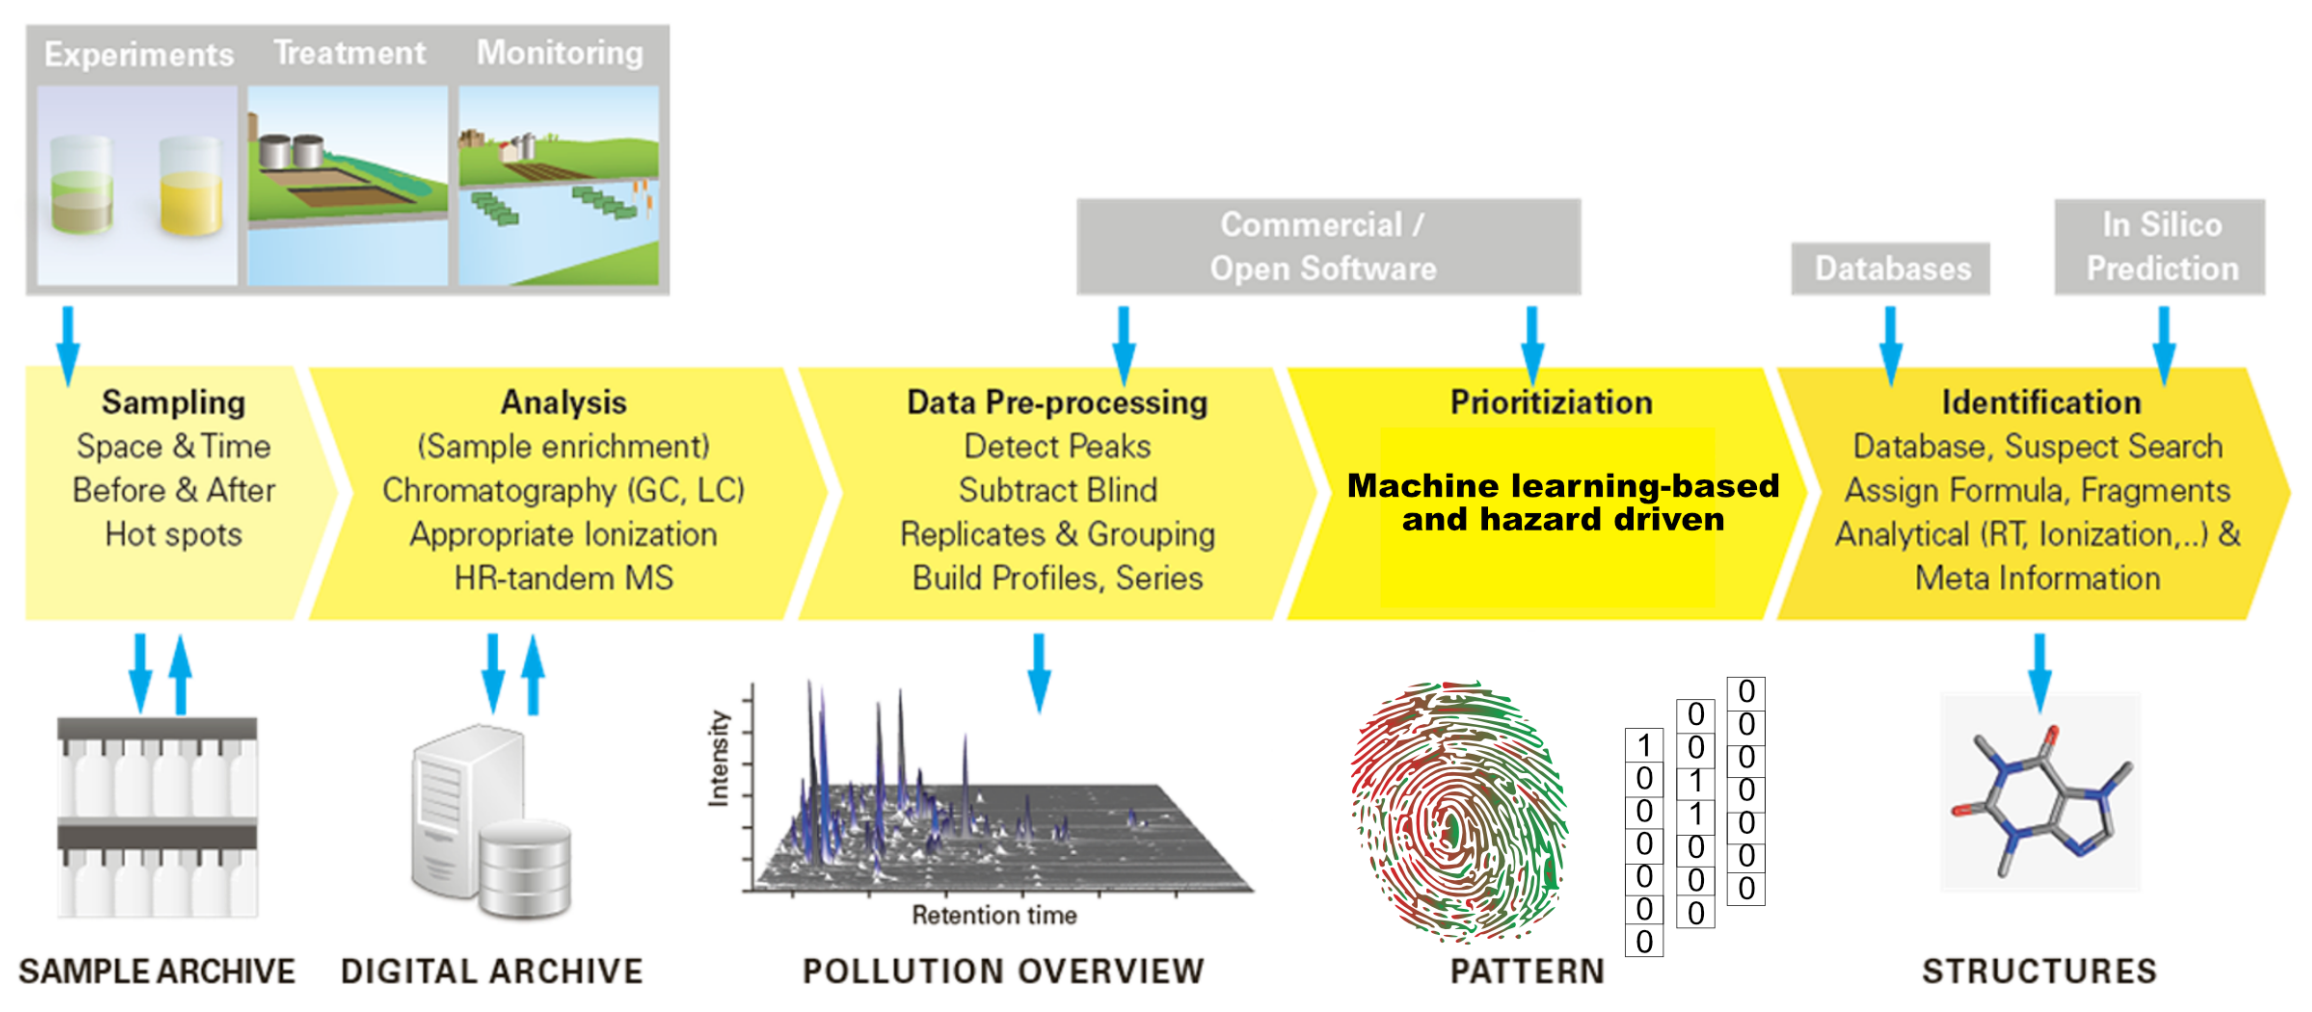
\includegraphics[width=1.0\textwidth]{figures/non_target_high_resolution_mass_spectrometry_1.png}  
    \caption{Figure 1 adapted (with modified Prioritization step) from Hollender et al.~\cite{hollender}: Nontarget screening with high resolution mass spectrometry in the environment: Ready to go? }
~\label{fig:non_target_high_resolution_mass_spectrometry} 
\end{figure}

\section{The Promise of Machine Learning in Toxicity Prediction}

In the past few years, machine learning has emerged as a transformative force in the field of toxicology, particularly in the realm of high-throughput toxicity prediction. High-throughput screening (HTS) has revolutionized the way we assess toxicity by allowing thousands of in vitro bioassays to be conducted rapidly. This high-throughput approach, coupled with advancements in robotics and automated analysis, has generated large volumes of toxicity data, paving the way for more comprehensive assessments of chemical compounds.
Alongside the rise of machine learning, this advancement has facilitated the creation of predictive models capable of forecasting compound toxicity based on their chemical structure. These models can be trained on extensive datasets containing well-documented toxicity information, allowing them to learn the underlying patterns and relationships between chemical structure and target toxicity. Once trained, these models can reliably predict the toxicity of new compounds, even if they have not undergone laboratory testing. This approach holds the potential to significantly reduce the time and cost associated with early-stage toxicity pre-assessment and plays a crucial role in prioritizing compounds for further in-depth testing.

\section{MLinvitroTox: A Novel Approach}

In response to the pressing need for a more hazard-driven and comprehensive assessment of environmental contaminants, Arturi et al. introduced MLinvitroTox~\cite{arturi}, an innovative machine learning framework. In particular it is the primary goal of this thesis to collaborate with the authors in further advancing and developing this framework. MLinvitroTox leverages molecular fingerprints extracted from fragmentation spectra~\footnote{also termed as Tandem mass spectrometry or MS/MS or MS2}, marking a fundamental shift in how we forecast the toxicity of the myriad unidentified HRMS/MS features. While traditional QSAR models predict bioactivities based on molecular fingerprints derived from chemical structures, MLinvitroTox was trained with supervised classification models on molcular fingerprints from chemical structures but is applied to molecular fingerprints generated from experimentally measured MS2 spectra using \emph{SIRIUS} and \emph{CSI:FingerID}. SIRIUS is a software package for annotating small molecules from nontarget HRMS/MS data, while CSI:FingerID is a machine-learning tool employed by SIRIUS to predict molecular fingerprints from fragmentation spectra. MLinvitroTox leverages streamlined machine learning techniques to predict the compounds bioactivity, respectively toxicity, ensuring a broad toxicological coverage encompassing nearly 300 target-specific and 90 cytotoxic endpoints, sourced from ToxCast/Tox21 data. Subsequently, the toxicity predictions generated by the framework are employed to prioritize compounds, with the flexibility to emphasize specific aspects of toxicity profiles tailored to individual preferences. This prioritization strategy facilitates more streamlined and thorough evaluations of environmental contaminants, enhancing a more hazard-driven risk assessment.





\section{Objectives and Significance}

The central objective of this thesis is to develop a streamlined framework for the prediction of compound toxicity across multiple endpoints, resulting in the creation of toxicity fingerprint. The generated toxicity fingerprints will provide valuable insights for the prioritization process in identifying most hazardous compounds found in environmental samples, ultimately contributing to the preservation of ecosystems and our health. The framework aims to develop a custom curation of structural and toxicological data to address challenges from modeling heterogenuous, and imbalanced data sets. Notably, the use of SIRIUS molecular fingerprints and xgboost (Extreme Gradient Boosting) models, complemented by feature selection?, has yielded consistently successful results. Furthermore, we have validated the effectiveness of MLinvitroTox by applying it to MassBank spectra, demonstrating an average balanced accuracy of 0.75? in predicting toxicity.

\section{Thesis Structure}

The initial chapters lay the groundwork by providing essential background information and summarizing related work. As we progress through the subsequent chapters, we will delve into the methodology and technical intricacies involved in preparing ToxCast/Tox21 toxicity data, transforming them into suitable inputs for our machine learning pipeline. This foundational work will serve as the cornerstone for the forthcoming chapters, where we will showcase the potential of MLinvitroTox. Additionally, will also demonstrate the framework's effectiveness through validation using real-world data and discuss about the implications of our research.
